\documentclass{article}
\usepackage{graphicx}
\usepackage[utf8]{inputenc}
\usepackage[T1]{fontenc}
\usepackage{pgfplots}
\usepackage{pgfplotstable} 
\usepackage{titlesec}
\usepackage{lipsum}
\usepackage{authblk}
\usepackage{algorithm}
\usepackage[noend]{algpseudocode}
\usepackage {tikz}
\usetikzlibrary {positioning}

\titleformat{\chapter}[display]{\normalfont\bfseries}{}{0pt}{\Large}

\begin{document}

\title{Projeto e Análise de Algoritmos: Trabalho Prático 1}
\author{João Mateus de Freitas Veneroso}
\affil{Departamento de Ciência da Computação da Universidade Federal de Minas Gerais}

\maketitle

\section{Introdução}

Este relatório descreve a implementação do trabalho prático 2 da disciplina Projeto e Análise de Algoritmos. 
O trabalho consistiu em resolver um problema de compartilhamento de viagens por meio de três paradigmas diferentes:
força bruta, programação dinâmica e algoritmos gulosos.

\section{Força Bruta}

O algoritmo de força bruta descrito abaixo é o mesmo implementado no Trabalho Prático 1.

O algoritmo \ref{alg:alg_1} implementa uma solução de força bruta para o problema de compartilhamento de viagens. 
Primeiro inicializa-se o benefício máximo $ b^* $ com um valor negativo, dessa
forma qualquer configuração válida vai proporcionar um benefício maior. A partir daí, no loop das linhas 5-10, para cada configuração
válida, calcula-se o benefício total e atualiza-se o valor de $ b^* $ se este benefício for maior do que qualquer um encontrado até então.
Além disso, a variável $ G_p^* $ guarda a configuração que proporcionou o maior benefício. Ao final do algoritmo, $ b^* $ guarda o valor 
do benefício máximo para o grafo $ G $ e $ G_p^* $ guarda a configuração que proporcionou este benefício. 

A complexidade deste algoritmo depende do número de configurações $ G_p $ diferentes e do custo da função $ ConstraintsAreValid $. O número de 
configurações $ G_p $ diferentes é $ 2^m $ para $ m $ igual ao número de arestas no grafo $ G $. Pois, cada aresta pode estar presente ou
não em $ G_p $ e nós queremos as combinações possíveis para todas as arestas m. O custo da função $ ConstraintsAreValid $ depende do número de 
arestas, pois, para cada aresta $ (u,v) $, temos de verificar se ela é a única aresta que sai do vértice $ u $, se o vértice $ v $ é um motorista
e se $ v $ possui espaço para acomodar todos os passageiros de $ u $. Como todas estas operações tem custo constante, a função $ ConstraintsAreValid $ 
tem custo $ O(m) $. Por último, a linha 7 calcula a soma dos pesos de todas as arestas também com custo $ O(m) $. Logo, 
a complexidade total do algoritmo é $ 2m2^m $ e o algoritmo é $ O(m2^m) $.

\begin{algorithm}
\caption{MaximizeBenefit}\label{euclid}
\begin{algorithmic}[1]
\Procedure{MaximizeBenefit}{G = (V,A)}

\State $ b^* \gets -1 $
\State $ G_p^* \gets \emptyset $
\item \ForAll{\textit{$ G_p = (V, A_p) : A_p \subseteq G.A $}}

\If {\textit{ConstraintsAreValid($G_p$)}}
  \State $ \textit{b} \gets \sum_{(v_i, v_j) \in A_p} B(v_i, v_j) $
  \If {$ b > b^* $}
    \State $ b^* \gets b $
    \State $ G_p^* \gets G_p $
  \EndIf
\EndIf
\EndFor
\EndProcedure
\end{algorithmic}
\label{alg:alg_1}
\end{algorithm}

Uma melhora ainda pode ser alcançada se deixarmos de testar parte das configurações inválidas de $ G $. Sabemos que 
um passageiro só pode pegar carona em uma rota, portanto, qualquer combinação $ G_p $ onde existirem arestas $ (u, v_i), (u, v_j) : i \neq j $
é inválida. Dessa forma, basta manter uma única aresta ativa por vez na lista de adjacência de cada vértice. Por exemplo, na figura \ref{fig:graph} apenas 
duas combinações precisam ser testadas: $ G_0(V,A_0) : A_0 = \{(X,Y)\} $ e $ G_1(V,A_1) : A_1 = \{(X,Z)\} $.

Além disso, é necessário lembrar que um vértice pode representar um motorista sem passageiros ou um passageiro que não vai pegar carona com ninguém, 
portanto, o número total de combinações 
se torna $ \sum_{v \in V} G \rightarrow Adj(v) + 2 $ e, no pior caso (um grafo completo), o número de combinações se torna $ O(n^n) $ 
onde n é o número de vértices no grafo $ G $. Feitas estas considerações, a complexidade assintótica do algoritmo é $ O(mn^n) $.
O algoritmo implementado em Python para este trabalho utiliza este método.

A complexidade de espaço do algoritmo original e da versão aprimorada é $ O(n + m) $, pois o grafo é armazenado na forma de listas de adjacência.

\section{Programação Dinâmica}

No problema do compartilhamento de viagens modelado em grafos, os vértices do grafo representam viagens e as arestas do grafo representam 
compartilhamentos. Para fins de simplificação da explicação, consideremos que os vértices podem representar passageiros exclusivos, motoristas exclusivos 
ou passageiros-motoristas. Em qualquer solução válida os passageiros-motoristas tem de decidir se vão
atuar como passageiros ou motoristas devido às restrições do problema. Dessa forma, sendo k o número de passageiros-motoristas, 
ao variar quais deles atuam como passageiros e quais atuam como motoristas, existem $ 2^k $ combinações possíveis que dão origem a problemas distintos. 
Cada um destes problemas pode ser pensado como um grafo bipartido G(V,A) onde os vértices de passageiros pertencem a um subconjunto de V e os vértices 
de motoristas pertencem a um outro subconjunto de V, sendo que todas as arestas conectam um vértice passageiro a um vértice motorista e os dois subconjuntos
são disjuntos.

\begin{figure}
  \center
  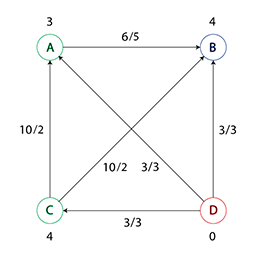
\includegraphics[width=128px]{graph.png}
  \caption{Exemplo do problema de compartilhamento de viagens modelado em forma de grafo}
  \label{fig:graph}
\end{figure}

\begin{figure}
  \center
  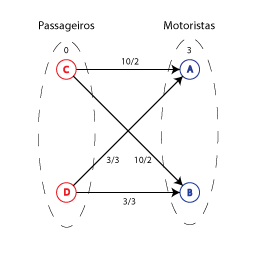
\includegraphics[width=164px]{bipartite_graph.png}
  \caption{Grafo bipartido após definição dos passageiros e motoristas no grafo da figura \ref{fig:graph}}
  \label{fig:bipartite_graph}
\end{figure}

A figura \ref{fig:graph} mostra um exemplo do probema de compartilhamento de viagens modelado na forma de um grafo, onde vértices
vermelhos representam grupos de passageiros, vértices azuis representam motoristas e vértices verdes representam passageiros-motoristas. Os números
próximos aos vértices representam a capacidade do veículo e os números próximos às arestas $ (v_i, v_j) $ representam o 
benefício do compartilhamento $ B(v_i, v_j) $ e o número de passageiros na viagem $ Q(v_i, v_j) $ separados por uma barra.
Perceba que os vértices A e C são passageiros-motoristas e os demais vértices são passageiros ou motoristas exclusivos. Ao selecionar 
o vértice A como motorista e o vértice C como passageiro, podemos modelar o problema com o grafo bipartido da figura \ref{fig:bipartite_graph}.
Para cada uma das combinações de passageiros e motoristas podemos construir um grafo bipartido similar. Nesta forma, o problema passa a se parecer
bastante com o \textit{0-1 Multiple Knapsack Problem}, com a diferença que alguns items podem estar restritos à sacolas específicas. No caso, as sacolas
representam os carros e os itens representam os grupos de passageiros. Ao definir a composição de benefício máximo para cada um destes problemas,
basta escolher a composição de maior benefício para obter uma solução ótima para o problema completo.

Digamos que existem $ n $ grupos de passageiros $ {p_1, p_2, ..., p_n} $ e $ m $ carros $ {c_1, c_2, ..., c_m} $ no grafo bipartido, 
sendo que $ |p_i| $ é o número de passageiros no grupo $ i $ e $ |c_j| $ é a capacidade máxima do carro $ j $. Agora, digamos
que $ P_i = \{ p_1, p_2, ..., p_i \} $, $ C_j = \{ c_1), C(c_2), ..., C(c_j) \} $ e $ B*(P_i, C_j, |c_j|) $ é o conjunto de arestas de 
benefício máximo para $ P_i $ e $ C_j $ onde a lotação do carro $ j $ é no máximo $ |c_j| $. Para calcular o 
valor de $ B*(P_i, C_j, |c_j|) $ temos três possibilidades:

\begin{enumerate}  
\item o grupo de passageiros $ p_i $ viajará no carro $ c_j $
\item o grupo de passageiros $ p_i $ viajará em algum carro no conjunto $ \{c_1, c_2, ..., c_{j - 1} \} $
\item o grupo de passageiros $ p_i $ não viajará em nenhum carro
\end{enumerate}

Se $ |p_i| > |c_j|$ ou a aresta $ (p_i, c_j) $ não existe no grafo bipartido, então o caso 1 é impossível. 
Caso contrário, o benefício máximo no caso 1 é $ B(p_i, c_j) + B*(P_{i-1}, C_j, |c_j| - |p_i|) $. Observe
que a capacidade do carro $ j $ agora é $ |c_j| - |p_i| $, pois ele está incorporando o grupo de passageiros 
$ p_i $ que possui $ |p_i| $ passageiros.

No caso 2, o benefício máximo é $ B*(P_{i}, C_{j-1}, |c_{j-1}|) $, pois o grupo de passageiros $ p_i $ não 
está indo no carro $ c_j $

o caso 1 é impossível

o benefício máximo será 

sendo que todo carro possui uma capacidade
sendo que toda aresta $ (p_i, c_j) $ liga um passageiro a um carro. 


Para cada aresta do grafo bipartido $ (v_i, v_j) $ que representa
O problema descrito acima Subestrutura ótima


sobreposição de subproblemas

K matrizes com P linhas e C colunas.
K = motoristas
P = passageiros (p1, p2, p3, ..., pn)
C = capacidade do carro



% Cada célula da matriz Kn[i][j] guarda o benefício máximo dado que os passageiros p1, p2, ..., p_i já foram alocados entre os carros k1, k2, ..., k_n. 
% 
% Para calcular Kn[i][j] primeiro colocamos o passageiro p_i no carro k_n e calculamos o beneficio desta escolha com a expressão p_i.benefit + Kn[i - 1][j - p_i.weight]. Sendo que, se i - 1 = 0 a expressão é somente p_i.benefit e se p_i.weight >= C_j a expressão é 0.
% 
% Tendo calculado o benefício, é necessário comparar a escolha com o benefício máximo em outras posições.
% 
% Primeiro, verificamos se Kn[i-1][j] tem um benefício maior. Nesse caso, não vale a pena colocar o passageiro p_i no carro. Ficamos com Kn[i-1][j].
% 
% Segundo, verificamos se Kn[i][j - 1] é maior.
% 
% Terceiro, temos que verificar se vale mais a pena colocar o passageiro em qualquer outro carro K_{n - 1}, K_{n - 2}, etc. Se K_{n - 1}[i][max_capacity] > Kn[i][j]. Ficamos com K_{n - 1}[i][max_capacity].
% 
% Podemos calcular as matrizes na seguinte ordem:
% 
% Para passageiros 1 a n
%     Para carros 1 a K
%        Para capacidades 0 a K_n.capacity
% 
% Resta provar que essa recursão garante sempre a melhor escolha.
% 
% Se 
% 
% Suponha que a aresta A pertence a solução de benefício máximo, mas k[i][j - A.weight]
% não é máximo. Então, seria possível achar uma configuração cujo valor seria maior do que k[i][j - A.weight], mas nesse caso poderíamos substituir essa configuração em k[i][j] gerando um benefício maior, mas nesse caso, k[i][j] não seria máximo o que contradiz nossa hipótese inicial.
% 
% Agora suponha que o passageiro não vai em nenhum outro carro e k[i-1][j] não é máximo. Então existe uma configuração em que o passageiro p_i não vai em nenhum carro cujo benefício máximo é maior do que k[i-1][j], mas nesse caso poderíamos substituir essa configuração em k[i][j] e o benefício seria maior, contradizendo a hipótese que k[i][j] era máximo.
% 
% Suponha que k[i][j] é uma configuração de benefício máximo e o passageiro p_i vai pegar carona com em um outro carro k_n e suponha que k_n[i][max_capacity] não tem benefício máximo. Nesse caso, como nos exemplos anteriores podemos tomar uma outra configuração onde max_benefit > k_n[i][max_capacity] e substituir em k[i][j] resultando em uma configuração de maior benefício máximo o que contradiz a hipótese que k[i][j] era uma configuração de benefício máximo.
% 
% Isso conclui a prova.
% 
% 
% Greedy
% Ordene os carros por capacidade
% Ordene os passageiros por beneficio / peso 
% Para cada carro, escolha os passageiros com maior razão benefício / peso até estourar o limite do carro.
% 
% Para provar que não chega na solução, basta tomar um grafo em q cada passageiro está ligado a um único carro e basta construir um exemplo que não chegue a um resultado otimo no 0-1 knapsack.
% 

\end{document}
